We have seen that even problems with multiple dimensions of
flexibility can be solved optimally in polynomial time.
In particular, we presented a dynamic program to
jointly optimize the node placement and (multiple)
chunk assignment, even under capacity
constraints ($\FP+\MA+\CC+\BW$), or an algorithm
to optimize the replica selection and assignment of multiple chunk types ($\RS+\MA+\CC+\BW$).

This section now points out fundamental
limitations in terms of computational tractability. In particular, we
will show that problems become NP-hard if multiple replicas have to be
assigned to a flexibly placeable node ($\FP+\RS+\MA$ is proved NP-hard in
Section~\ref{ssec:fprsma}), and if inter-connects have to be established
between flexible nodes ($\FP+\RS+\CC$ is proved NP-hard in Section~\ref{ssec:fprscc}); both
results hold even in uncapacitated networks, and even in small-diameter
substrate networks (namely two- or three-level trees~\cite{fattree}).
The hardness of $\FP+\RS+\MA$ and $\FP+\RS+\CC$ imply
the hardness of four additional, more general models, as
summarized in the following figure:

\begin{figure}[htbp]
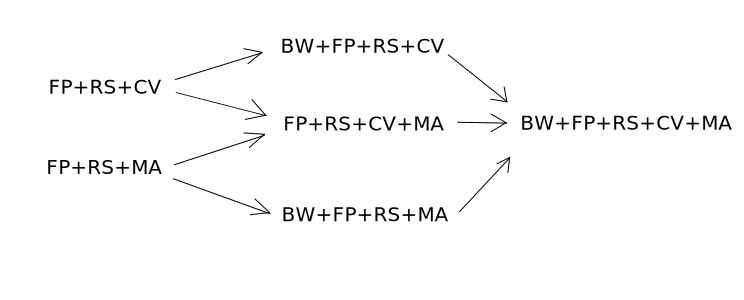
\includegraphics[width = \columnwidth]{figs/np-hierarchy}
\end{figure}


\subsection{Introduction to 3D Perfect Matching}

Both the hardness of $\FP+\RS+\MA$ and $\FP+\RS+\CC$ is shown by a reduction
from the NP-complete problem of \emph{3D Perfect Matching}~\cite{3dmatch},
which
can be seen as a generalization of bipartite matchings to 3-uniform
hypergraphs. We will refer to this problem by $\TDM$, and for completeness,
review it in the following.

$\TDM$ is defined as follows. We are given three finite and disjoint
sets $X$, $Y$, and $Z$ of cardinality $k$, as well as a subset of triples $T\subset
X \times Y \times Z$.  Set $M \subseteq T$ is a 3-dimensional matching
if and only if, for any two distinct triples $(x_1, y_1, z_1) \in M$
and $(x_2, y_2, z_2) \in M$, it holds that $x_1\neq x_2$, $y_1\neq
y_2$, and $z_1\neq z_2$. Our goal is to decide if we can construct
a $M \subseteq T$ which is \emph{perfect}, that is, a subset which covers all
elements of $X \times Y \times Z$.

TODO: cite Karp on result of NP-completeness
TODO: image like this: \url{https://upload.wikimedia.org/wikipedia/commons/thumb/5/50/3-dimensional-matching.svg/240px-3-dimensional-matching.svg.png}

\subsection{Multi-Assignments are hard ($\FP+\RS+\MA$)}\label{ssec:fprsma}

Our proof that $\FP+\RS+\MA$ is NP-hard is based on the following main ideas.
We encode an $\TDM$ instance as an $\FP+\RS+\MA$ instance as follows:

 \begin{itemize}
 \item For every element in the universe $X\cup Y\cup
 Z$, we create a chunk type. Intuitively, in $\TDM$,
 each element must be covered, which corresponds to the requirement
 of $\FP+\RS+\MA$,
 that each chunk type is processed.

 \item We will encode each triple as three leaves in
 a substrate tree $\Tree$. The three leaves are close to each
 other in $\Tree$, and the placement of chunk replicas in $\FP+\RS+\MA$
 corresponds to the elements of the
 triples in these leaves.

 \item The node placement will correspond to choice of triples,
 independently in which leaf the node is mapped.
 A node will process the chunk which is located on the same server,
 as well as the chunks in other two leaves of the same gadget.

\item We will use threshold cost to ensure that no node
will process
any chunk outside its gadget.
\end{itemize}

\textbf{Construction.}
Given an instance $I$ of $\TDM$, we construct an instance $I'$ of
$\FP+\RS+\MA$ as follows:
\begin{itemize}
\item \emph{Tree Construction:} We create a tree consisting of a root,
and for each triple, we create a gadget which we directly attach as
child of the root. The gadget is of height 2,
and has the following form:
The gadget of each triple $T_i$ consists of an inner node (a router) and three leaves.
\item \emph{Chunks and chunk replicas:} For each element in $X$, $Y$ and $Z$,
 we create a chunk type
($3 \cdot k$ in total). Every gadget
contains three chunk replicas, corresponding to the elements of $T_i$.
\item \emph{Other properties:} We set the number of to-be-embedded nodes to $k$,
$\CostTrans$ to $1$, and the number of slots in each node to $m=3$ \stefan{what
is the number of slots here?}. We use a threshold $\Thr=2 \cdot 2 \cdot k$.
\end{itemize}

The construction is illustrated in Figure~\ref{fig:fprsma}.
\begin{figure}[htbp]
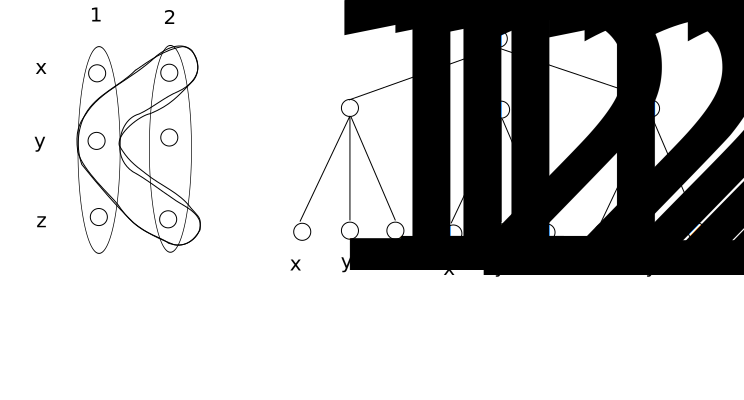
\includegraphics[width = \columnwidth]{figs/example-matching}
\end{figure}
\stefan{TODO: finish picture and add a caption explaining its elements}


\textbf{Correctness.}
Given these concepts, we can now show the computational hardness.
\begin{theorem}
$\FP+\RS+\MA$ is NP-hard.
\end{theorem}
\begin{proof}
Let $I$ be an instance of $\TDM$ and let $I'$ be an instance of
$\FP+\RS+\MA$ constructed as described above.
We prove that $I'$ has solution of cost $\leq \Thr$ if ($\Rightarrow$) and only if
($\Leftarrow$)
$I$ has a matching of size $k$.

($\Rightarrow$) Let us take a solution to $\TDM$. We place a node in every
gadget that corresponds to the chosen triples. We match every chunk in a
gadget to a node in this gadget (only the chosen ones). This solution has
cost exactly $\Thr$. As every element of the universe is covered, every
chunk type is processed.

($\Leftarrow$) Let us take a solution to $\FP+\RS+\MA$ of cost $\leq \Thr$. We
choose triples that correspond to gadgets where there are nodes. Since
all chunks are processed, very element of $X$, $Y$ and $Z$ is matched. Each
node must processes chunks that correspond to the triple, otherwise the
cost must be larger than $\Thr$ (high costs for the connection between
nodes and chunks).
\end{proof}


\subsection{Inter-connects are hard ($\FP+\RS+\CC$)}\label{ssec:fprscc}

Next, we prove that the joint optimization of node placement and replica selection
is NP-hard if an inter-connect has to be established between virtual machines.
In our terminology, this is the $\FP+\RS+\CC$ problem.

\textbf{Construction.}
Concretely, let $I$ be an instance of $\TDM$. We will create an instance $I'$
for $\FP+\RS+\CC$ as follows:
\begin{itemize}
\item We will construct the same tree as in previous reduction with
chunk replicas placed in the same way.
\item We set the access cost $\CostTrans$ to a chunk replica to a high value $W$. This will force
nodes to be collocated with the replica.
(For now, we can assume that $W=\infty$; a lower and sufficient bound will be given
in the Appendix.)
\item The communication cost in the inter-connect is set to $\CostCom = 1$.
\item The number of nodes (virtual machines) is $\Vms = 3 \cdot k$.
\item We use a threshold $\Thr =  6 \cdot k + 3 \cdot 3 \cdot 2 \cdot
(k - 1) \cdot k$.
\end{itemize}


\textbf{Proof of correctness.}
Intuitively, in order to minimize embedding costs,
nodes should be placed on near-by replicas. We use the following
helper lemma.
\begin{lemma}\label{lemma:helper}
In every valid solution $\Sol$ of $I'$ of cost $\leq \Thr$, each gadget
falls in one of two categories:
$k$ gadgets have exactly
$3$ nodes, and $n-k$ gadgets remain empty.
\end{lemma}
\begin{proof}
Since $W=\infty$, nodes will always be placed
directly on chunks (the access network cost is zero).
Moreover, since
$\Sol$ is valid, $3 \cdot k$ nodes are mapped
directly to the different chunk locations.
Now, consider any pair of nodes communicating over the
inter-connect; due to our construction, the communication cost
for each such pair is either
2 hops (if they belong to the same gadget) or 4 hops (if they belong
to different gadgets).
The lemma then follows from the observation that $\Thr$
is chosen such that it is never possible to distribute nodes
among more than $k$ gadgets.
\end{proof}

\begin{theorem}
$\FP+\RS+\CC$ is NP-hard.
\end{theorem}
\begin{proof}
Let $I$ be an instance of $\TDM$ and let $I'$ be an instance of
$\FP+\RS+\CC$ constructed as described above.
We prove that $I'$ has solution of cost $\leq \Thr$ if ($\Rightarrow$) and only if
($\Leftarrow$)
$I$ has a solution.

($\Rightarrow$) In order to compute a solution
for $I'$ given a solution for $I$, we proceed as follows.
Given a covering set of triples $S = \{T_1, T_2, \ldots, T_k\}$, we place three nodes in each gadget that
corresponds to every triple of $S$. Chunks are matched to nodes that are located
on the same server.

The solution has the following cost:
(1) the communication cost inside a gadget is $2 \cdot {3 \choose 2}$,
  as every pair contributes two hops;
  (2) the communication cost from each gadget to all other gadgets is $4
  \cdot 3 \cdot 3 \cdot (k - 1) / 2$, where the factor $4$ is
  for the
  communication over $4$ hops, the factor $3$
  corresponds to the number of nodes per gadget, and
  $3 \cdot (k-1)$ is the number of nodes in remote gadgets;
  as we count each pair twice, we need to divide by two in the end.
Summing up over all $k$ gadgets, we get exactly $\Thr$.

($\Leftarrow$) Given a solution for $I'$,
we can exploit Lemma~\ref{lemma:helper} to construct a solution for $I$.
We know that in any solution of cost at most $\Thr$,
$k$ gadgets contain exactly 3 nodes. These gadgets correspond to a valid
3D Perfect Matching: every
chunk was processed and hence every element in the $X \cup Y \cup Z$ is covered.
\end{proof}

